\section{Baseline Plan}
Figure \ref{baselineplan} shows our initial baseline plan. Although this plan indicates that we will follow a procedure that resembles the waterfall method, meaning that we always take steps in one direction, we expect that we will revisit some phases again if we feel that some knowledge or information is lacking.

In the initiation phase, we will familiarize with the potential project by identifying the key stakeholders, figuring out the future vision of the proposed project and get introduced to the steering committee. In the in-line phase, we will connect the visions and the goals of the design project to DMA’s current business and IT strategies. This includes interviews and workshops with the creators of the online courses and identifying all the possible domains of the project. The in-depth phase will then look at the current working practices of the previously identified domains. Example of this might be analysing how the doctors use the system both at work and in their spare time. Finally, the innovation phase will be used to finish the design project report along with the creation of prototypes and mockups to demonstrate the use and ideas of the proposed system.

\begin{figure*}
 \begin{center}
  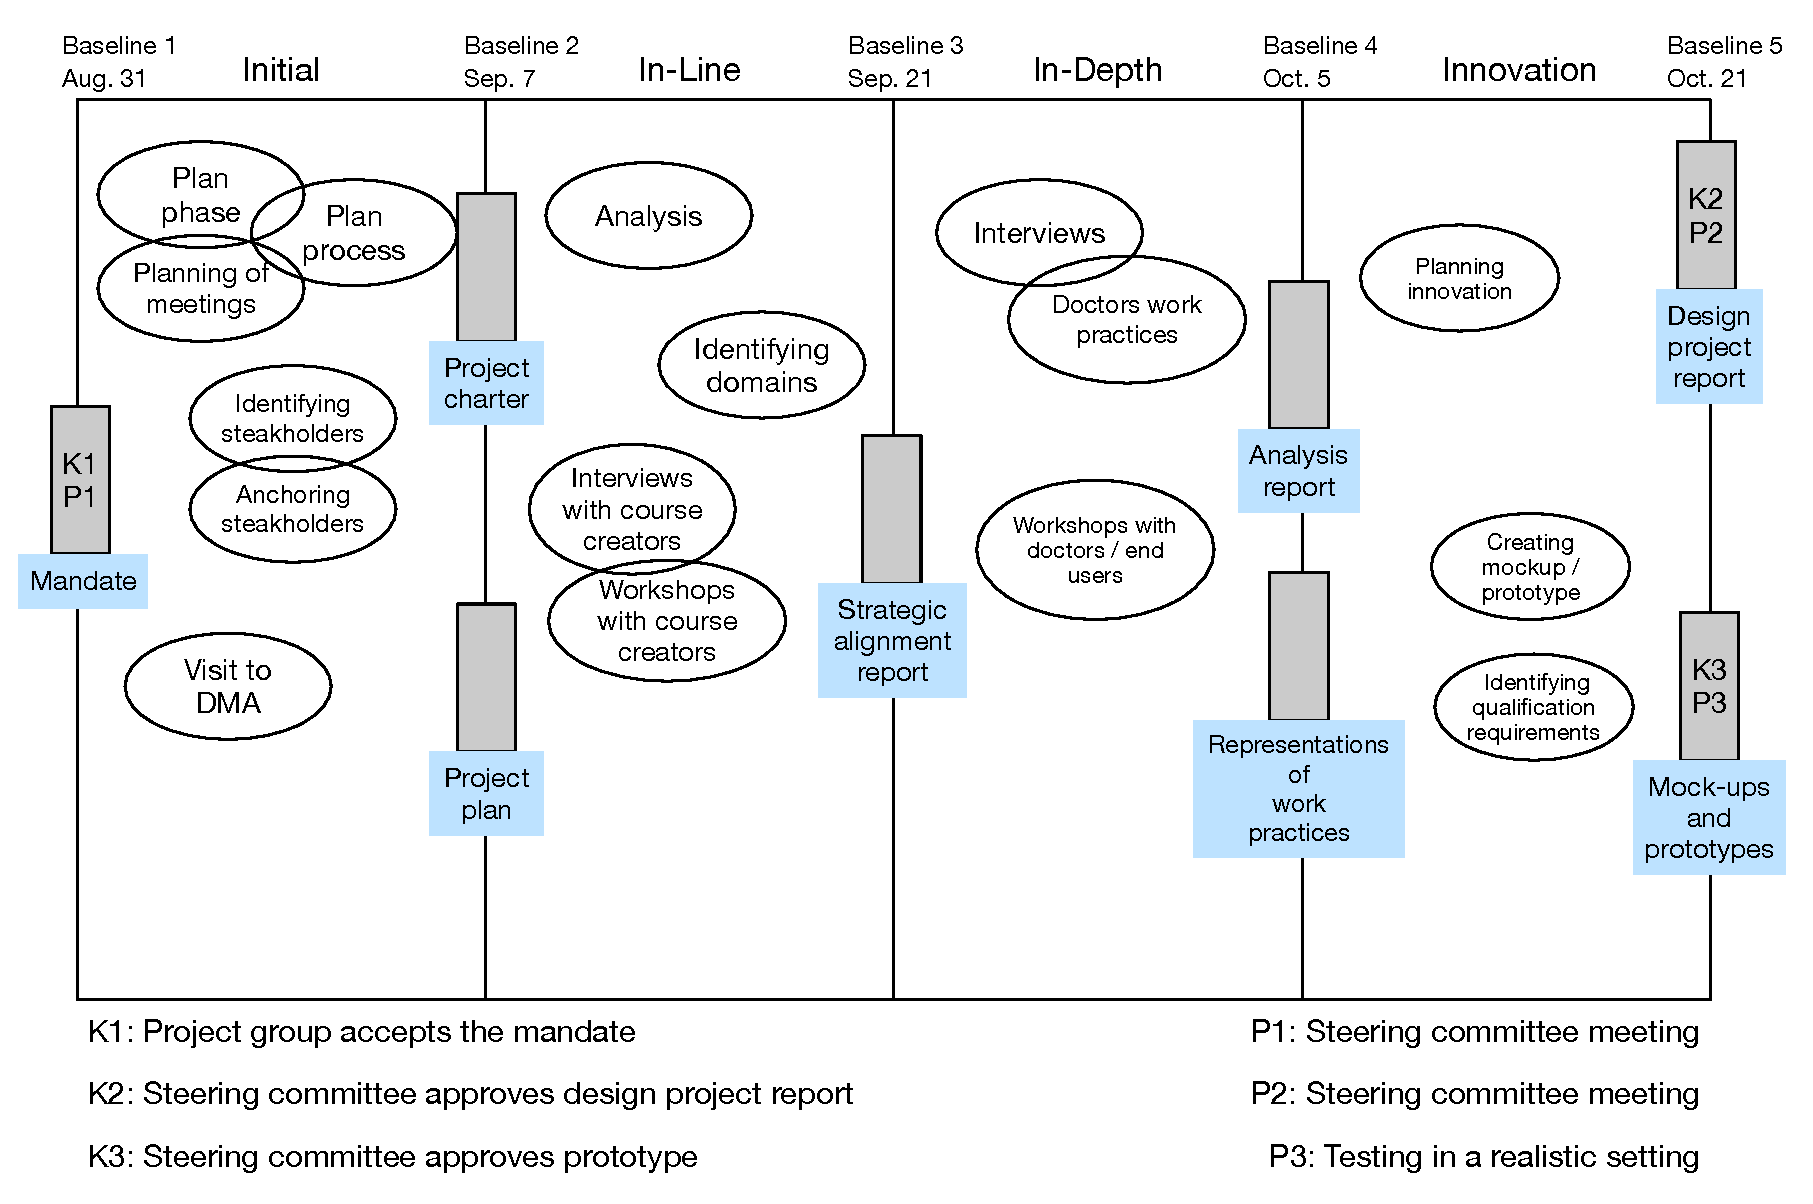
\includegraphics[width=1\textwidth]{figures/baseline-plan.pdf}
  \caption{Our baseline plan for the project.\label{baselineplan}}
 \end{center}
\end{figure*}

